\documentclass[tikz,border=10pt]{standalone}

\usetikzlibrary{
    arrows.meta,
    positioning,
    calc,
    fit,
    backgrounds,
    shapes.geometric
}

\definecolor{rxnblue}{HTML}{2B6CB0}
\definecolor{rxnpurple}{HTML}{6B46C1}
\definecolor{rxnorange}{HTML}{DD6B20}
\definecolor{rxngreen}{HTML}{2F855A}
\definecolor{rxnred}{HTML}{C53030}
\definecolor{textgray}{HTML}{2D3748}

\begin{document}

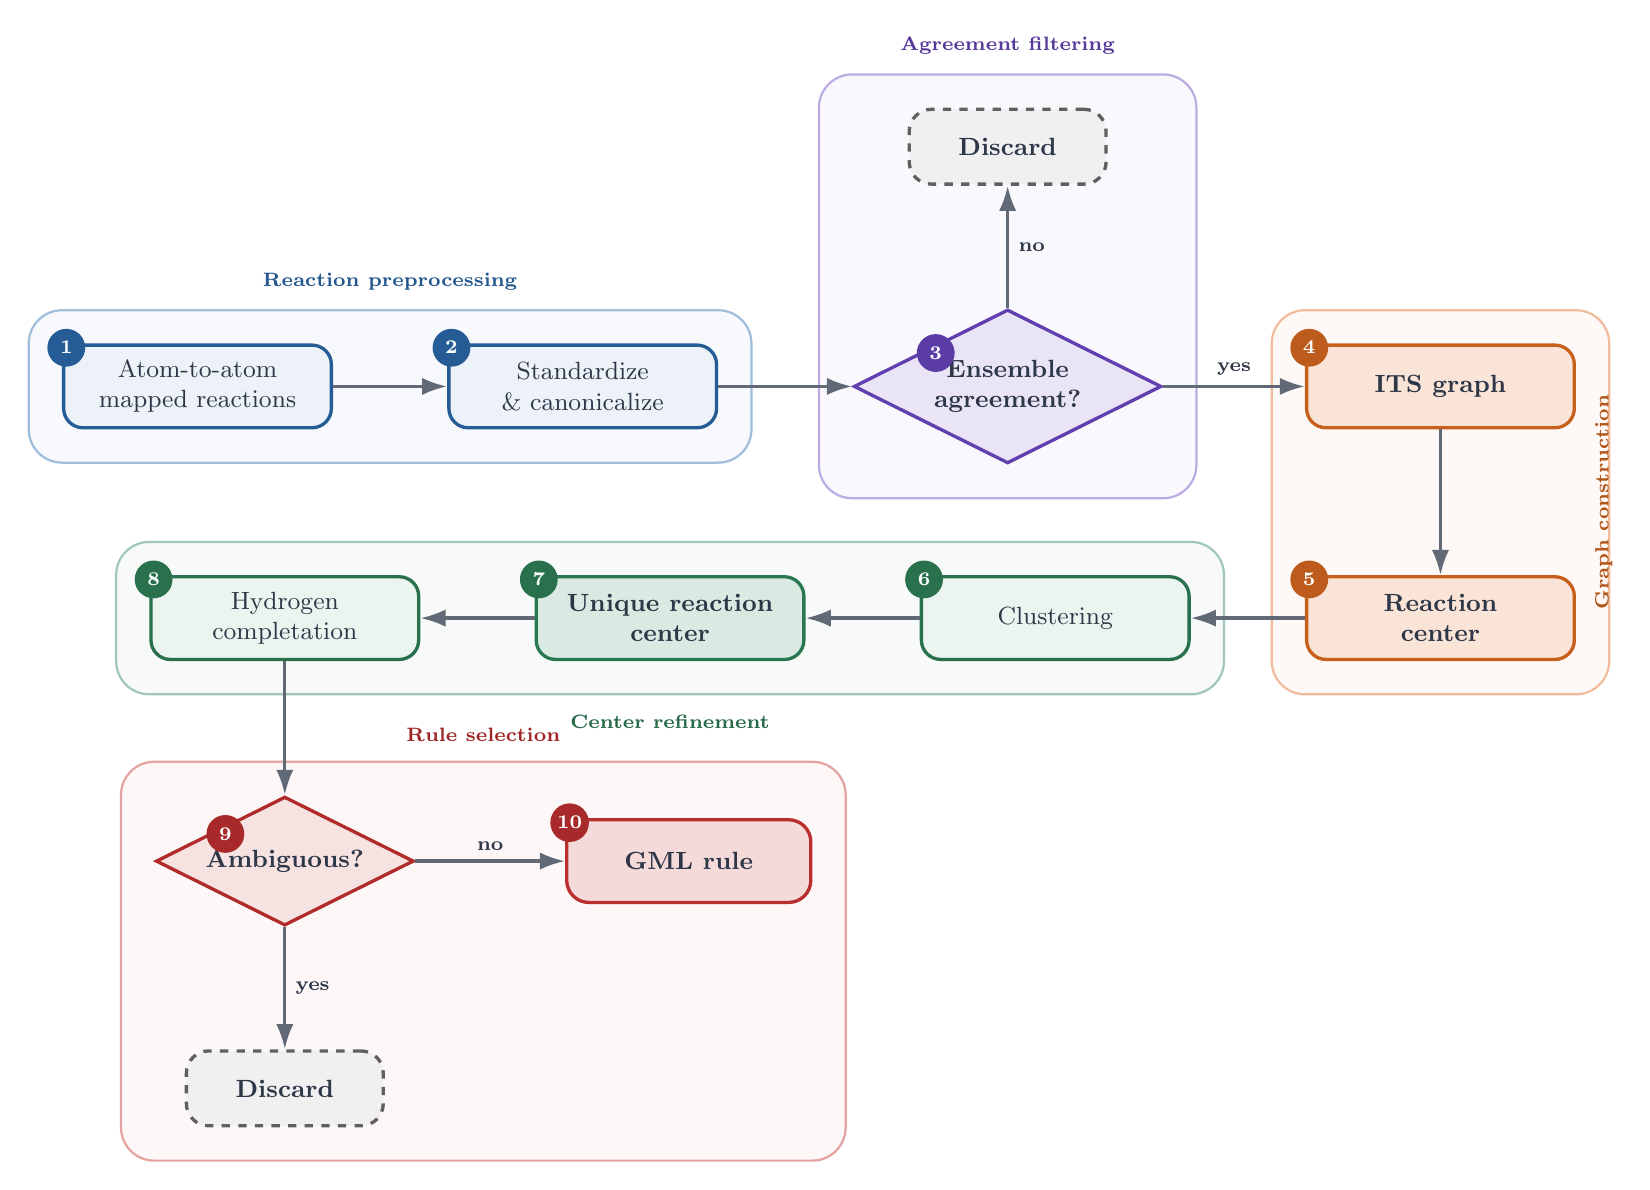
\begin{tikzpicture}[
    font=\sffamily,
    node distance=1.45cm and 1.45cm,
    every node/.style={text=textgray},
    step/.style={
        rectangle,
        rounded corners=7pt,
        minimum width=3.4cm,
        minimum height=1.05cm,
        align=center,
        font=\small,
        very thick,
        draw=#1!85!black,
        fill=#1!9
    },
    core/.style={
        rectangle,
        rounded corners=7pt,
        minimum width=3.4cm,
        minimum height=1.05cm,
        align=center,
        font=\small\bfseries,
        very thick,
        draw=#1!90!black,
        fill=#1!18
    },
    decision/.style={
        diamond,
        aspect=2.0,
        minimum width=2.9cm,
        minimum height=1.25cm,
        align=center,
        font=\small\bfseries,
        very thick,
        draw=#1!90!black,
        fill=#1!14
    },
    output/.style={
        rectangle,
        rounded corners=8pt,
        minimum width=3.1cm,
        minimum height=1.05cm,
        align=center,
        font=\small\bfseries,
        very thick,
        draw=#1!95!black,
        fill=#1!18
    },
    discard/.style={
        rectangle,
        rounded corners=8pt,
        minimum width=2.5cm,
        minimum height=0.95cm,
        align=center,
        font=\small\bfseries,
        draw=gray!75!black,
        fill=gray!12,
        very thick,
        dashed
    },
    arrow/.style={
        -{Latex[length=3.2mm,width=2.2mm]},
        very thick,
        draw=textgray!75
    },
    phase/.style={
        rectangle,
        rounded corners=12pt,
        draw=#1!45,
        fill=#1!4,
        thick,
        inner xsep=12pt,
        inner ysep=12pt
    },
    phaselabel/.style={
        font=\scriptsize\bfseries,
        text=#1!80!black
    },
    number/.style={
        circle,
        inner sep=1.4pt,
        minimum size=4.8mm,
        font=\scriptsize\bfseries,
        text=white,
        fill=#1!85!black
    }
]

% =====================================================
% Top row
% =====================================================

\node[step=rxnblue] (aam)
{Atom-to-atom\\mapped reactions};

\node[step=rxnblue, right=of aam] (std)
{Standardize\\\& canonicalize};

\node[decision=rxnpurple, right=1.7cm of std] (agree)
{Ensemble\\agreement?};

\node[discard, above=1.55cm of agree] (discard1)
{Discard};

\node[core=rxnorange, right=1.8cm of agree] (its)
{ITS graph};

% =====================================================
% Bottom row
% =====================================================

\node[core=rxnorange, below=1.85cm of its] (center)
{Reaction\\center};

\node[step=rxngreen, left=of center] (cluster)
{Clustering};

\node[core=rxngreen, left=of cluster] (unique)
{Unique reaction\\center};

\node[step=rxngreen, left=of unique] (hydrogen)
{Hydrogen\\completation};

\node[decision=rxnred, below=1.7cm of hydrogen] (ambiguous)
{Ambiguous?};

\node[output=rxnred, right=1.9cm of ambiguous] (gml)
{GML rule};

\node[discard, below=1.55cm of ambiguous] (discard2)
{Discard};

% =====================================================
% Arrows
% =====================================================

\draw[arrow] (aam) -- (std);
\draw[arrow] (std) -- (agree);

\draw[arrow] (agree) -- node[above, font=\scriptsize\bfseries] {yes} (its);
\draw[arrow] (agree) -- node[right, font=\scriptsize\bfseries] {no} (discard1);

\draw[arrow] (its) -- (center);
\draw[arrow] (center) -- (cluster);
\draw[arrow] (cluster) -- (unique);
\draw[arrow] (unique) -- (hydrogen);
\draw[arrow] (hydrogen) -- (ambiguous);

\draw[arrow] (ambiguous) -- node[above, font=\scriptsize\bfseries] {no} (gml);
\draw[arrow] (ambiguous) -- node[right, font=\scriptsize\bfseries] {yes} (discard2);

% =====================================================
% Number badges
% =====================================================

\node[number=rxnblue, anchor=north west] at ($(aam.north west)+(-0.12,0.12)$) {1};
\node[number=rxnblue, anchor=north west] at ($(std.north west)+(-0.12,0.12)$) {2};
\node[number=rxnpurple, anchor=north west] at ($(agree.north west)+(-0.10,0.10)$) {3};
\node[number=rxnorange, anchor=north west] at ($(its.north west)+(-0.12,0.12)$) {4};
\node[number=rxnorange, anchor=north west] at ($(center.north west)+(-0.12,0.12)$) {5};
\node[number=rxngreen, anchor=north west] at ($(cluster.north west)+(-0.12,0.12)$) {6};
\node[number=rxngreen, anchor=north west] at ($(unique.north west)+(-0.12,0.12)$) {7};
\node[number=rxngreen, anchor=north west] at ($(hydrogen.north west)+(-0.12,0.12)$) {8};
\node[number=rxnred, anchor=north west] at ($(ambiguous.north west)+(-0.10,0.10)$) {9};
\node[number=rxnred, anchor=north west] at ($(gml.north west)+(-0.12,0.12)$) {10};

% =====================================================
% Background phase boxes
% =====================================================

\begin{scope}[on background layer]
    \node[phase=rxnblue, fit=(aam)(std)] (p1) {};
    \node[phase=rxnpurple, fit=(agree)(discard1)] (p2) {};
    \node[phase=rxnorange, fit=(its)(center)] (p3) {};
    \node[phase=rxngreen, fit=(cluster)(unique)(hydrogen)] (p4) {};
    \node[phase=rxnred, fit=(ambiguous)(gml)(discard2)] (p5) {};
\end{scope}

% =====================================================
% Phase labels
% =====================================================

\node[phaselabel=rxnblue, above=0.12cm of p1.north]
{Reaction preprocessing};

\node[phaselabel=rxnpurple, above=0.12cm of p2.north]
{Agreement filtering};

\node[phaselabel=rxnorange, right=0.15cm of p3.east, rotate=90, anchor=south]
{Graph construction};

\node[phaselabel=rxngreen, below=0.12cm of p4.south]
{Center refinement};

\node[phaselabel=rxnred, above=0.12cm of p5.north]
{Rule selection};

\end{tikzpicture}

\end{document}